% !TeX spellcheck = en_US
\addsection{AI rules}{\spells/fortune.png}

\begin{multicols}{2}

  AI rules apply to enemy heroes and all Combats, including against Neutral armies, in \textbf{Solo Campaigns} and \textbf{Cooperative} Scenarios.

  \pagetarget{AI Heroes}{\subheader{AI Heroes}}
  AI Heroes are used in the Campaigns.
  Their units are static and are defined by the Scenario: find the indicated unit cards when you start the scenario.
  If the unit indicates unit tier (\svg{bronze}, \svg{silver}, \svg{golden}, or \svg{azure}) instead of ``Few'' or ``Pack'', that's a Neutral Unit.

  During setup, if multiple AI Heroes use the same unit, and you do not have enough copies of its card, the AI Heroes must share it:
  set everything up without that card, and add it to the AI Hero's Army the moment you trigger Combat with them.

  AI Heroes cannot surrender and you cannot surrender to them;
  they will always fight until they run out of units.
  Winning Combat against an AI Hero does not grant any rewards unless stated by the Scenario.
  AI Heroes do not have a Town Board, Resources, or a Hero Board.

  \columnbreak
  \subsection*{AI Heroes Turns}
  Unless specified otherwise, AI heroes start in their Town, take turns after the player, and have 3 MP, always spending them to perform the following Actions in descending priority:
  \begin{itemize}
    \item If a player's Hero is on the same Tile as the AI, spend all MP to move towards them in an attempt to start Combat.
    \item If there are any Mines or Settlements the AI could flag on the same Tile, move towards the closest one.
    \item Otherwise, move toward the player's Town.
  Repeat this sequence until all MPs are used up.
  AI Heroes take their turn after the player.
  \end{itemize}

  AI Heroes always \textbf{automatically win Combat} against any Neutral Units, while simultaneously \textbf{flagging or Visiting all Fields} they happen to move through.
  They gain no benefits from any Fields.

  AI Heroes must discover face down Map Tiles as normal by spending 1 MP before moving onto them.
  The player chooses that Tile's orientation.
\end{multicols}

{\begin{center}
    \includegraphics[width=\linewidth,height=\textheight,keepaspectratio]{\art/harpy.jpg}
\end{center}}

\pagetarget{AI Deck}{\subheader{AI Decks}}
\begin{multicols*}{2}
  \begin{tikzpicture}
    \node (card) {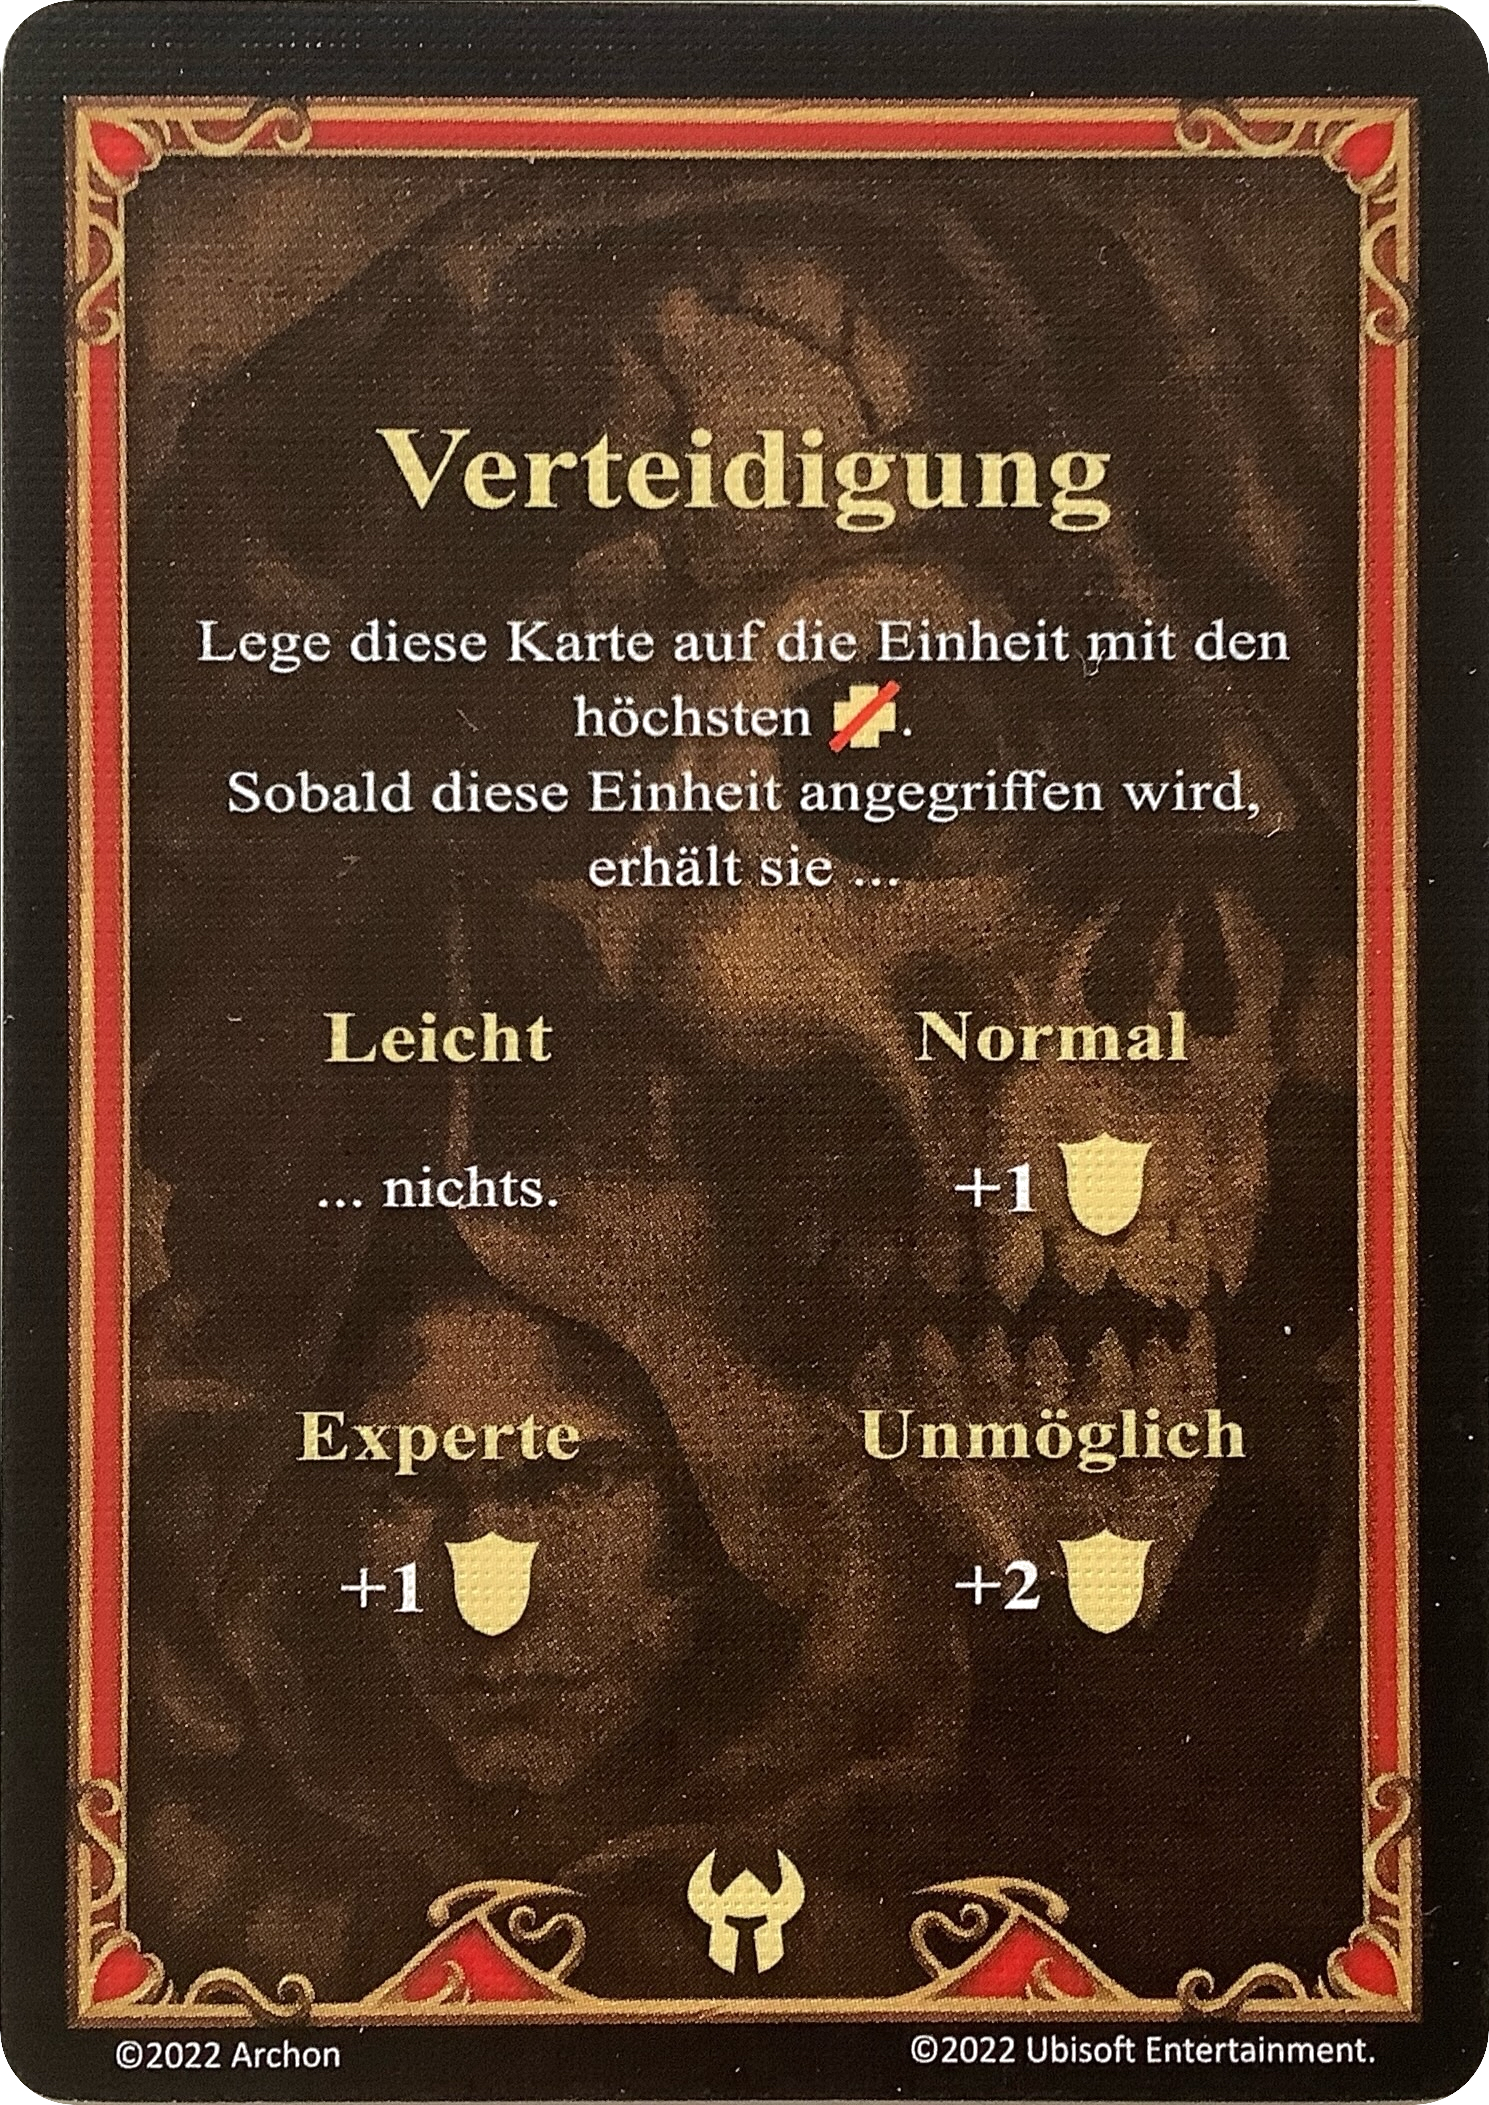
\includegraphics[width=0.57\linewidth]{\cards/ai.png}};
    \begin{scope}[
      shift={(card.south west)},
      x={($(card.east) - (card.west)$)},
      y={($(card.north) - (card.south)$)},
      ]
      \draw (0.4, 0.85) node {\encircle{1}};
      \draw (0.8, 0.7) node {\encircle{2}};
      \draw (0.15, 0.5) node {\encircle{3}};
      \draw (0.55, 0.5) node {\encircle{4}};
      \draw (0.15, 0.3) node {\encircle{5}};
      \draw (0.55, 0.3) node {\encircle{6}};
      \draw (0.4, 0.1) node {\encircle{7}};
    \end{scope}
    \node [below=0pt of card.south] {\imagecaption{AI card}};
    \node [right=0pt of card.east] {
      \begin{minipage}[t]{0.47\linewidth}
        \scriptsize
        \begin{itemize}[itemsep=0.8em]
          \item[\textbf{1.}] Name
          \item[\textbf{2.}] Description
          \item[\textbf{3.}] Easy Modifier
          \item[\textbf{4.}] Normal Modifier
          \item[\textbf{5.}] Expert Modifier
          \item[\textbf{6.}] Impossible\\Modifier
          \item[\textbf{7.}] Card Type:\\
            \begin{itemize}[itemsep=0.5em]
              \item[\svg{might}] Might
              \item[\svg{magic}] Magic
              \item[\svg{skill}] Skill
            \end{itemize}
        \end{itemize}
      \end{minipage}
    };
  \end{tikzpicture}

  AI Heroes use two Decks during Combat: the \textbf{AI Deck}, and the \textbf{AI Spell Deck}.
  The AI Deck consists of three types of AI cards: Might \svg[12]{might}, Magic \svg{magic} and Skill \svg{skill}.
  Each Campaign Scenario lists the number and types of cards to include during setup.
  Choose these cards \textbf{randomly} when building the AI Deck.
  Shuffle the AI Deck before each Combat together with its discard pile.

  When an AI Hero \textbf{activates} a unit, draw an AI card\index{AI card} and follow its instructions before the unit \pagelink{AI Units}{moves and/or attacks}.
  If AI Deck is depleted during Combat, stop drawing from it.
  The effect of each AI card depends on the game's \pagelink{Difficulty}{Difficulty}.
  If an AI Hero is instructed to draw a card, they will draw and resolve \textbf{another card} from the AI Deck.

  If an AI card increased a unit's \svg{defense}, or triggered another card which increased it, the AI card stays attached to the unit until the first defense happens.
  % TODO: why attack isn't mention in expansion book? is it not the case for attack?
  % our old text here: The Might card \svg[12]{might} is attached to the unit until the first respective attack/defense happens.

  \subsection*{AI Deck sharing}
  If there are multiple AI Enemy Armies in the Scenario, but the rules don't specify which Enemy an AI Deck, an AI Spell Deck, or a Skill belongs to, you should assume it is shared between them.

  \subsection*{AI Magic cards and AI Spell Deck}
  Build the \textbf{AI Spell Deck} by separating the indicated Spells from the regular Spell Deck during setup.
  Shuffle the AI Spell Deck before each Combat together with its discard pile.

  Whenever an AI Magic \svg{magic} card is drawn, draw the next spell from the the AI Spell Deck, and cast it.
  Discarded spells go to its own AI Spell Discard pile.
  If the AI Spell deck empties before Combat ends, shuffle the AI Spell discard pile to form a new Spell deck.

  Sometimes in the AI Spell deck, there are more Spell cards than there are Magic cards in the AI Hero's deck.
  This is no mistake: not all spells need to be used, some are there for the sake of diversity.

  If the AI Hero is assigned a Spell card that is unavailable because it's your Hero's Deck, and you don't have another copy, substitute it with a \wikilink{spells/magic_arrow}{Magic Arrow} card.

  For certains spells it can be unclear how AI is supposed to use them.
  See \pagelink{AI Complex Spells}{Casting Complex Spells} for explanations.

  \subsection*{AI Skill cards}
  If Skill cards are included, search for and set aside the indicated card related to it (usually, an Ability).
  Whenever an AI Hero uses the AI Skill \svg{skill} card, use the skill card assigned to them in the Setup, but do not discard it afterwards.
  Contrary to the regular rules, the AI Hero can use the skill again, when instructed to do so by the AI deck.
  Discard the AI Skill \svg{skill} card as usual.

  AI Skill cards cannot be replaced, so if setup assigns the AI Hero a card that your Hero has and you don't have another copy,
  remove the needed card from your Hero's deck and \textbf{Search (3)} the respective card's deck to compensate your Hero for the loss.
\end{multicols*}

\pagetarget{AI Units}{\subheader{Combat against AI}}
\begin{multicols*}{2}
  These rules apply during Combat in \textbf{Solo}\index{Solo Mode} and \textbf{Cooperative} Scenarios.
  The rules for AI unit placement during setup are described in \pagelink{CombatAISetup}{Combat section}.

  When Neutral enemies or AI Heroes activate a unit, they follow a set of automatic instructions:\par

  \begin{itemize}
    \item If it's an AI Hero, draw and resolve the next \pagelink{AI Deck}{AI card}.

    \item Enemy Ground \svg{unit_ground} and Flying \svg{unit_flying} units prioritize attacking units of the \textbf{same} tier.
    If this is impossible, they attack the unit of a lower tier (in tier \textbf{descending} order, down to bronze), and if that is also impossible, they attack the unit of a higher tier (in tier \textbf{ascending} order).\par

    \textit{Example: \svg{golden}\svg{unit_ground} has this priority:
    \svg{golden}
    - \svg{silver}
    - \svg{bronze}
    - \svg{azure}.}

    \item Ranged \svg{unit_ranged} units prioritize attacking other Ranged \svg{unit_ranged} units of the same tier, then lower tier, and finally higher tier, using the same tier order as above.
    If there are no Ranged \svg{unit_ranged} units for them to target, they prioritize Ground \svg{unit_ground} and Flying \svg{unit_flying} units in the same tier order.\par

    \textit{Example: \svg{silver}\svg{unit_ranged} has this priority:
    \svg{silver}\svg{unit_ranged}
    - \svg{bronze}\svg{unit_ranged}
    - \svg{golden}\svg{unit_ranged}
    - \svg{azure}\svg{unit_ranged}
    - \svg{silver}\svg{unit_ground}\svg{unit_flying}
    - \svg{bronze}\svg{unit_ground}\svg{unit_flying}
    - \svg{golden}\svg{unit_ground}\svg{unit_flying}
    - \svg{azure}\svg{unit_ground}\svg{unit_flying}.}
  \end{itemize}

  In both cases, if there's more than one valid target, they attack the closest one.
  If there's ever a tie between equally valid targets, the player chooses which unit is attacked.\par

  Enemy units cannot \pagelink{Defend}{defend} unless instructed to.

  \columnbreak
  \subsection*{AI Siege}
  When the Walls and Gate are mentioned in Combat preparation but no additional information on how to arrange them is given, arrange them just like a human player would:
  place the Gate in front of the \svg{unit_ground} unit with the highest \svg{initiative}.
  By default, the units do not attack the Walls -- they would rather fly over them to attack their target or move towards it through the Gate.
  If it is not possible, they take a \pagelink{Defend}{Defend} Action.

  The \pagelink{Walls}{Arrow Tower} is treated like a Silver \svg{silver}\svg{unit_ranged} unit.
  However, if there are multiple equally valid targets, it will attack the target closest to perishing (has the smallest difference between \svg{health_points} and current \svg{damage}).

  \vspace*{\fill}

\end{multicols*}

\pagetarget{AI Complex Spells}{\subheader{Casting complex spells}}
\begin{multicols*}{2}
  In some campaigns enemies use a number of spells whose effects are not fully compatible with the standard use of AI Magic \svg{magic} cards.
  To fully use their effects, here are extended descriptions of how AI Heroes should use each of these spells.
  Of course, the scenario can override this.

  \subsection*{Spells attacking multiple targets}
  \textit{Examples: \wikilink{spells/fireball}{Fireball,} \wikilink{spells/chain_lightning}{Chain Lightning.}}

  When activated, target any unit with one or two adjacent units from the player’s army, prioritizing the groups where there are more higher-tier units.
  If there is more than one valid group, attack the one that is between the closest to perishing (has the smallest difference between \svg{health_points} and current \svg{damage}).
  If there is still more than one valid target, then you can choose which unit is attacked.
  If there are no player units adjacent to one another, target units that are not adjacent to any of the AI units.
  If that is also not possible, do not use this spell -- instead, skip the AI \svg{magic} card that activated this effect and put it on the bottom of the Enemy AI deck, then shuffle this spell back to the Enemy Spell deck.

  \subsection*{Instant Defense spells}
  \textit{Example: \wikilink{spells/stone_skin}{Stone Skin.}}

  When activated, put this card on the side of the Combat board, then put a Defense token on the unit with the highest \svg{defense} to represent the card’s effect -- it stays there until the defense is resolved.
  If there already is a Defense token on that unit, choose another one in the order of decreasing \svg{defense}.
  In case of a tie in \svg{defense} value, give preference to the unit of the highest tier and then to the greatest value of \svg{damage}.

  \columnbreak
  \subsection*{Healing spells}
  \textit{Example: \wikilink{spells/cure}{Cure.}}

  When activated, remove the \svg{damage} from the AI unit with the greatest value of \svg{damage} tokens, starting with the highest tier available.
  If no AI unit has any \svg{damage}, put the AI \svg{magic} card that triggered the spell at the bottom of the Enemy AI deck, then shuffle this Spell card back to the Enemy Spell Deck.

  \subsection*{Single-round buffs}
  \textit{Example: \wikilink{spells/fire_shield}{Fire Shield.}}

  % TODO FIFO or LIFO? do they all activate at the same time during first unit next round?
  When activated, check the tier of the unit on which you are about to cast the spell and count how many units of the same or higher tier there are on the board.
  If more than half of them have already activated this turn, do not cast the spell now -- instead, place it on the side of the Combat board and play it when the first AI unit activates in the next combat round.
  Skip drawing the AI card for that activation.

  \subsection*{Attack-weakening spells}
  \textit{Example: \wikilink{spells/weakness}{Weakness.}}

  When activated, if the AI’s activated unit is about to perform an attack that will provoke a Retaliation, cast this spell on the Retaliating enemy to lower their \svg{attack}.
  If the AI’s unit causes no Retaliation, do not cast this spell -- instead, ignore the AI card that activated the spell and put it at the bottom of the Enemy AI deck, then shuffle the Spell card back to the Enemy Spell deck.
\end{multicols*}
